%%%%%%%%%%%%%%%%%%%%%%%%%%%%%%%%%%%%%%%%%
% Beamer Presentation
% LaTeX Template
% Version 1.0 (10/11/12)
%
% This template has been downloaded from:
% http://www.LaTeXTemplates.com
%
% License:
% CC BY-NC-SA 3.0 (http://creativecommons.org/licenses/by-nc-sa/3.0/)
%
%%%%%%%%%%%%%%%%%%%%%%%%%%%%%%%%%%%%%%%%%

%----------------------------------------------------------------------------------------
%	PACKAGES AND THEMES
%----------------------------------------------------------------------------------------

\documentclass{beamer}

\mode<presentation> {

% The Beamer class comes with a number of default slide themes
% which change the colors and layouts of slides. Below this is a list
% of all the themes, uncomment each in turn to see what they look like.

%\usetheme{default}
%\usetheme{AnnArbor}
%\usetheme{Antibes}
%\usetheme{Bergen}
%\usetheme{Berkeley}
%\usetheme{Berlin}
%\usetheme{Boadilla}
%\usetheme{CambridgeUS}
%\usetheme{Copenhagen}
%\usetheme{Darmstadt}
%\usetheme{Dresden}
%\usetheme{Frankfurt}
%\usetheme{Goettingen}
%\usetheme{Hannover}
%\usetheme{Ilmenau}
%\usetheme{JuanLesPins}
%\usetheme{Luebeck}
\usetheme{Madrid}
%\usetheme{Malmoe}
%\usetheme{Marburg}
%\usetheme{Montpellier}
%\usetheme{PaloAlto}
%\usetheme{Pittsburgh}
%\usetheme{Rochester}
%\usetheme{Singapore}
%\usetheme{Szeged}
%\usetheme{Warsaw}

% As well as themes, the Beamer class has a number of color themes
% for any slide theme. Uncomment each of these in turn to see how it
% changes the colors of your current slide theme.

%\usecolortheme{albatross}
%\usecolortheme{beaver}
%\usecolortheme{beetle}
%\usecolortheme{crane}
%\usecolortheme{dolphin}
%\usecolortheme{dove}
%\usecolortheme{fly}
%\usecolortheme{lily}
%\usecolortheme{orchid}
%\usecolortheme{rose}
%\usecolortheme{seagull}
%\usecolortheme{seahorse}
%\usecolortheme{whale}
%\usecolortheme{wolverine}

%\setbeamertemplate{footline} % To remove the footer line in all slides uncomment this line
%\setbeamertemplate{footline}[page number] % To replace the footer line in all slides with a simple slide count uncomment this line

%\setbeamertemplate{navigation symbols}{} % To remove the navigation symbols from the bottom of all slides uncomment this line
}

\usepackage{graphicx} % Allows including images
\usepackage{booktabs} % Allows the use of \toprule, \midrule and \bottomrule in 
%----------------------------------------------------------------------------------------
%	TITLE PAGE
%----------------------------------------------------------------------------------------
 
\usepackage{lmodern, textcomp}


\title[BST 234 Lab 2]{BST 234 - Lab 2} % The short title appears at the bottom of every slide, the full title is only on the title page

\author{Divy Kangeyan} % Your name
\institute[ ] % Your institution as it will appear on the bottom of every slide, may be shorthand to save space
{
  \\ % Your institution for the title page
\medskip
\textit{ } % Your email address
}
\date{\today}%\date{\today} % Date, can be changed to a custom date

\begin{document}

\begin{frame}
\titlepage % Print the title page as the first slide
\end{frame}

 

%----------------------------------------------------------------------------------------
%	PRESENTATION SLIDES
%----------------------------------------------------------------------------------------
 
 \begin{frame}
\frametitle{An interesting book on numbers}
 

 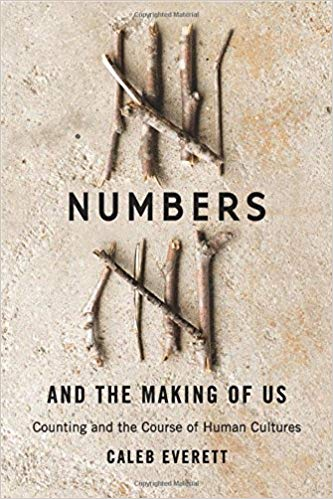
\includegraphics[width=2 in, height=3 in]{Numbers_book.jpg}

\end{frame}
 
 
 
\begin{frame}
\frametitle{Run time complexity}
 
$$f \in O(g) : \exists \ c>0, \ \exists n_{0} \ s.t. \ \forall \ n>n_{0} : f (n) \le  c*g(n)$$
 
\vspace{1.3cm}
Intuitively this means f (n) is O(g(n)) if f (n) grows at most as fast
as some constant times g(n) for large n. 

%\begin{center}
%\includegraphics[width=5cm]{plotOn.png}
%\end{center}

This is read as `'f(x) is big-Oh of g(x)" or `'g asymptotically dominates f."
 

\end{frame}



\begin{frame}
\frametitle{Properties}

\begin{itemize}
\item f= O(f) % f shorthand for f(n)
\item O(O(f)) = O(f)
\item kO(f) = O(f)
\item O(f + k) = O(f)
\item O(f) + O(g) = O(max(f , g))
\item O(f) $*$ O(g) = O(f $*$ g)
\end{itemize}

\end{frame}

 

\begin{frame}
\frametitle{Exercise 1}
 \textbf{Show that}: $$n^{2} \ is \ not\  in\ O(n) $$\\
 
\

\end{frame}

\begin{frame}
\frametitle{Exercise 1}
 \textbf{Show that}: $$n^{2} \ is \ not\ in\ O(n) $$\\
 
\textbf{Solution:} Suppose $\exists$ constants c and
$n_{o}$ for which: $$n^{2}\leq cn, \forall \ n > n_{o} $$ 
by \textit{dividing} both sides of the inequality \textit{by n},
then $n\leq c$ must hold $\forall \ n>n_{o}$.   \\

A contradiction!

\end{frame}


\begin{frame}
\frametitle{Exercise 2}
\textbf{Show that }: $$2^{n+1} \in O(2^n)$$ \\
 

\end{frame}


\begin{frame}
\frametitle{Exercise 2}
\textbf{Show that }: $$2^{n+1} \in O(2^n)$$ \\
 
\textbf{Solution:} $$2^{n+1}\leq 2^n*2 \ , \forall n\geq 0 $$ 
 $$\therefore \ 2^{n+1}=O(2^n)$$

\end{frame}
 

\begin{frame}
\frametitle{Exercise 3}
\textbf{Show that}: $$2^{2n}\ is \ not\ in\ O(2^n)$$\\
 


\end{frame}

\begin{frame}
\frametitle{Exercise 3}
\textbf{Show that}: $$2^{2n}\ is \ not \ O(2^n)$$\\
 
\textbf{Solution}: If the above was true,there would exist $n_{0}$ and c such that $n>n_{0}$ :
$$2^{n}*2^{n} =2^{2n} \leq c*2^n  $$ ,
so $2^{n}\leq c$ for $n>n_{0}$ which is clearly impossible since c is a constant. 
%$ \nexists c:2^{n}*2^{n} \leq c*2^{n}$. 

\end{frame}


\begin{frame}
\frametitle{Run -Time Complexity - Alternate Definition}
 

Assume g(n) $\ne $ 0 near $\infty$. \\

$$f \in O(g) \iff   \limsup\limits_{n\rightarrow \infty} \frac{f(n)}{g(n)} < \infty  $$ 

$$\limsup\limits_{n\rightarrow \infty} h(n) = \lim\limits_{n\to \infty} \Big (\sup_{m\geq n} h(m) \Big)$$ 

  (i.e. the limit of the least upper bound) 
 
\end{frame}
%------------------------------------------------
 
 


\begin{frame}
\frametitle{f in O(g)? some examples:}
 $$\lim_{n \to \infty} \frac{n}{2n}  = \frac{1}{2}, \ n \
 is \ O(2n)$$\\
 
  $$\lim_{n \to \infty} \frac{2n}{n}  = 2, \ 2n \ is \ O(n)$$ \\
  
  $$\lim_{n \to \infty}  \frac{ n}{\sqrt[]{n} } \to \infty, \ n \ is \ not \ O(\sqrt[]{n} )$$  
  

  \end{frame}

\begin{frame}
\frametitle{Exercise 4}
\textbf{Prove:} $$log(log(n))=O(log^{2}n)$$
 



{\color{blue}\textbf{Hint: L'Hospital's rule} }
\vspace{2cm}
  
\end{frame}

\begin{frame}[noframenumbering]
\frametitle{Exercise 4}
\textbf{Prove:} $$log(log(n))=O(log^{2}n)$$

 
  $$\lim_{n \to \infty} \frac{log(log(n))}{log^{2}n}= $$
 
\end{frame}

\begin{frame}[noframenumbering]
\frametitle{Exercise 4}
\textbf{Prove:} $$log(log(n))=O(log^{2}n)$$

 
  $$\lim_{n \to \infty} \frac{log(log(n))}{log^{2}n}=\lim_{n \to \infty} \frac{\frac{1}{nlog(n)}}{\frac{2log(n)}{n}}=  $$

\end{frame}

 \begin{frame}[noframenumbering]
 \frametitle{Exercise 4}
\textbf{Prove:} $$log(log(n))=O(log^{2}n)$$

 
  $$\lim_{n \to \infty} \frac{log(log(n))}{log^{2}n}=\lim_{n \to \infty} \frac{\frac{1}{nlog(n)}}{\frac{2log(n)}{n}} = \frac{1}{2log^{2}n}=0$$
 

$$\therefore log(log(n))=O(log^{2}n)$$
 
\end{frame}

\begin{frame} 
 \frametitle{Exercise 5}
\textbf{Prove:}  $$\lim_{n \to \infty}    \frac{2^{n+1} - 1}{2^{n}}  \ is \  O(1)$$   
\end{frame}

\begin{frame}[noframenumbering]
 \frametitle{Exercise 5}
\textbf{Prove:}  $$\lim_{n \to \infty}    \frac{2^{n+1} - 1}{2^{n}}  \ is \  O(1)$$  

\textbf{Solution:}  $$\lim_{n \to \infty}    \frac{2^{n+1} - 1}{2^{n}} =\lim_{n \to \infty}   \frac{2^{n+1} * log(2)}{2^{n}*log(2)}=2 = O(1) $$\end{frame}

\begin{frame}
\frametitle{Exercise 6}
\begin{columns}[c] % The "c" option specifies centered vertical alignment while the "t" option is used for top vertical alignment

\column{.45\textwidth} % Left column and width
\textbf{Order from lowest to highest: }
\begin{enumerate}[I]
\item O($log_{10}$ n)
\item  O(n!) 
\item O($2^{n}$) 
\item O(1) 
\item O($log_{2}$ n) 
\item O(nlog n) 
\item O($n^{2}$) 
\item O(n)
\end{enumerate}

\column{.5\textwidth} % Right column and width
\begin{enumerate}

\item   O(1) 
\pause
\item O($log_{10}$ n)=O($log_{2}$ n)
\pause
\item   O(n) 
\pause
\item  O(nlog n) 
\pause
\item  O($n^{2}$)  
\pause
\item  O($2^{n}$)
\pause
\item  O(n!)
\end{enumerate}
\end{columns}
\end{frame}


\begin{frame}
\frametitle{  The `'=" sign in Big-Oh Notation}

$$n = O(n^{4})$$ 
$$n^{2} = O(n^{4})$$
$$n^{3} = O(n^{4})$$
$$\implies n = n^{2} = n^{3}$$ \\


The `'=" sign should be interpreted as a $\le$.

\end{frame}


\begin{frame}
\frametitle{ The `'="  sign in Big-Oh Notation}
\begin{center}
Is there an analog for $<$?
\end{center}
\end{frame}


\begin{frame}
\frametitle{Little-Oh Notation}

Assume g(n) $\neq$0 near $\infty$. 
$$f \in o(g) \iff   \limsup\limits_{n\rightarrow \infty} \frac{f(n)}{g(n)} = 0 $$ 

$$\limsup\limits_{n\rightarrow \infty} h(n) = \lim\limits_{n \to \infty} \Big (\sup_{m\geq n} h(m) \Big)$$ 

  (i.e. the limit of the least upper bound) 
\end{frame}

\begin{frame}
\frametitle{What's the Difference?}
{\color{green}True} for \textbf{Big-Oh but} \alert{not Little-Oh}:\\
\begin{itemize} 
\item $x^{3} \in O(x^{3})$ 
\item $x^{3} \in O(x^{3}+x)$ 
\item $x^{3} \in O(10x^{3})$ 
\end{itemize} 

{\color{green}True} for \textbf{Little-Oh}:
\begin{itemize} 
\item $x^{2} \in o(x^{3})$ 
\item $x^{3} \in o(x^{4})$ 
\item $x^{3} \in o(x!)$ 
\end{itemize} 
\end{frame}

 

\begin{frame} 
\frametitle{Exercise 7}
\textbf{Prove:} $n^{k} \in O(b^{n})$ and $b^{n} 	\notin O(n^{k}) \forall b> 1, n>1, k\geq 0$ \\
 \begin{center}
{\color{blue} \textbf{Hint}: use the following theorem: \\

Let f(n), g(n) be two non-negative functions. Then: $$\lim_{n \to \infty} \frac{f(n)}{g(n)} = 0 \implies f (n) \in O(g(n)) \ and \ g(n) 	\notin O(f(n))$$ }

\end{center}
\textbf{Use L'Hospitals! }


\end{frame}

\begin{frame}[noframenumbering]
\frametitle{Exercise 7}
\textbf{Prove:} $n^{k} \in O(b^{n})$ and $b^{n} 	\notin O(n^{k}) \forall b> 1, n>1, k\geq 0$ \\
 
 \begin{center}
{\color{blue} \textbf{Hint}: use the following theorem: \\

Let f(n), g(n) be two non-negative functions. Then: $$\lim_{n \to \infty} \frac{f(n)}{g(n)} = 0 \implies f (n) \in O(g(n)) \ and \ g(n) 	\notin O(f(n))$$ }
\end{center}
\textbf{Use L'Hospitals! }

$$\lim_{n \to \infty}  \frac{n^{k}}{b^{n}}= \lim_{n \to \infty}  \frac{kn^{k-1}}{log(b)b^{n}}
= \cdots \lim_{n \to \infty} \frac{k!} {b^{n}(log (b))^{k}}$$

\end{frame}

 

\begin{frame}
\frametitle{Insertion sort}

\begin{columns}[c]  
\column{.6\textwidth} % Left column and width
 
\begin{enumerate}
\item Input an unsorted array A of length n
\item Iterate from i=2:n
\item Remove element i
\item Compare with sorted elements$<$i
\item Insert element i in sorted position
\end{enumerate}

\column{.5\textwidth} % Right column and width
%\includegraphics[width=5cm]{insertion.jpg}
\end{columns}
 

\end{frame}





\begin{frame}
\frametitle{Exercise 8}
What is the worst-case runtime complexity of the insertion sort?Prove it. Best case?\\

{\color{blue}$$Hint: \ \sum_{n=1} i=\frac{n^{2}+n}{2}$$}
  
\end{frame}

\begin{frame} [noframenumbering]
\frametitle{Exercise 8}
What is the worst-case runtime complexity of the insertion sort? Prove it. Best case?
 \\
 \vspace{1cm}
 
Solution: $O(n^{2})$. Note that we execute the outer loop n times and in the worst case scenario, we must make i comparisons each iteration. Combine this with the hint on the previous slide. Best case is O(n).

\end{frame}

 
 
%------------------------------------------------

 

 
 
\end{document}